\RequirePackage{luatex85,shellesc}
\documentclass[tikz, convert={outext=.svg, command=\unexpanded{pdf2svg \infile\space\outfile}}]{standalone}
\usepackage{luaotfload}
\usepackage{xcolor}
\usepackage{microtype}
\usepackage{fontspec}
\usepackage{unicode-math}
\colorlet{mainlevel}{black}
\UseMicrotypeSet[protrusion]{basicmath}
\defaultfontfeatures{Ligatures=TeX, Scale=MatchLowercase}
\setmainfont{Source Serif Pro}
\setmathfont{Libertinus Math}

\usetikzlibrary{arrows,calc,shapes.callouts}
\tikzset{
  level/.style = {
    line width=4.0pt
  },
  connect/.style = {
    line width=2.0pt,
    dashed
  },
  energylevels class/.style={
    every text node part/.style={
      align=center,
      font={\LARGE}
    }
  },
  atomlabel class/.style={
    every text node part/.style={
      align=center,
      font={\huge}
    }
  },
}

\begin{document}

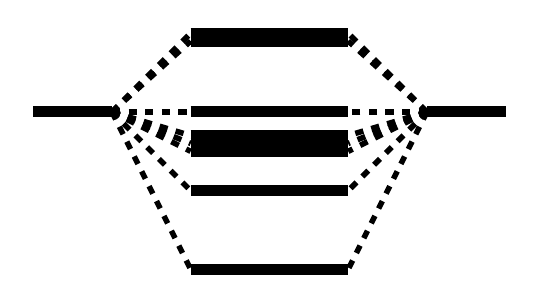
\begin{tikzpicture}

  \foreach \energy/\elevelbegin in {
    2/1,
    2/6
  } {
    \pgfmathsetmacro\elevelend{\elevelbegin + 1}
    \draw[level] (\elevelbegin,\energy) -- (\elevelend,\energy);
  }
  
  \foreach \energy/\elevelbegin in {
    0/3,
    1/3,
    1.5/3,
    1.6/3,
    1.7/3,
    2/3,
    2.9/3,
    3/3
  } {
    \pgfmathsetmacro\elevelend{\elevelbegin + 2}
    \draw[level] (\elevelbegin,\energy) -- (\elevelend,\energy);
  }
  
  \foreach \xbegin/\ybegin/\xend/\yend in {
    2/2/3/0,
    2/2/3/1,
    2/2/3/1.5,
    2/2/3/1.6,
    2/2/3/1.7,
    2/2/3/2,
    2/2/3/2.9,
    2/2/3/3,
    6/2/5/0,
    6/2/5/1,
    6/2/5/1.5,
    6/2/5/1.6,
    6/2/5/1.7,
    6/2/5/2,
    6/2/5/2.9,
    6/2/5/3
  } {
    \draw[connect] (\xbegin,\ybegin) -- (\xend,\yend);
  }
  
\end{tikzpicture}

\end{document}
